\documentclass{article}
\usepackage[a4paper,margin=2cm]{geometry}
\usepackage{amsmath}
\usepackage{tikz}
\usetikzlibrary{calc}
\usepackage{float}

\title{Spiral Theodorus dengan TikZ}
\author{Gunanto}
\date{\today}

\begin{document}
\maketitle

Spiral Theodorus dibangun dari segitiga siku-siku berantai: segitiga pertama
punya dua kaki sepanjang 1, sehingga sisi miringnya $\sqrt{2}$. Sisi miring itu
menjadi kaki segitiga berikutnya (kaki pendek tetap 1, tetap tegak lurus),
sehingga sisi miring baru $\sqrt{3}$, dan seterusnya. Sudut kumulatif dari
pusat bertambah $\arctan(1/\sqrt{n})$ pada segitiga ke-$n$.

\begin{figure}[H]
\centering
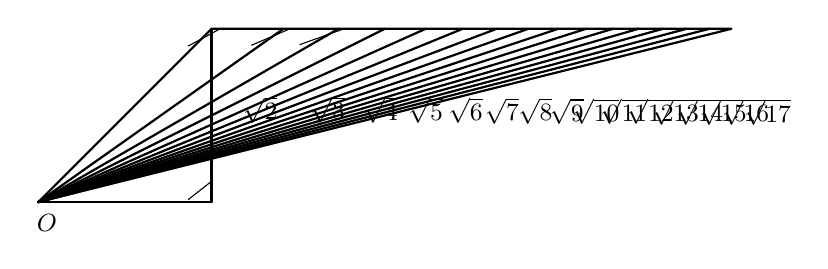
\begin{tikzpicture}[scale=2.2, line cap=round]
  \pgfmathsetmacro{\angleAcc}{0}
  \coordinate (O) at (0,0);
  \coordinate (P) at (1,0);
  \draw[thick] (O) -- (P);
  \foreach \n in {1,...,16}{
    \pgfmathsetmacro{\step}{atan2(1, sqrt(\n))}
    \pgfmathsetmacro{\angleAcc}{\angleAcc + \step}
    \pgfmathsetmacro{\r}{sqrt(\n+1)}
    \coordinate (Q) at ({\r*cos(\angleAcc)},{\r*sin(\angleAcc)});
    \draw[thick] (O) -- (Q);
    \draw[thick] (P) -- (Q);
    \pgfmathsetmacro{\midang}{\angleAcc - \step/2}
    \pgfmathsetmacro{\midr}{(\r + sqrt(\n))/2 + 0.18}
    \node[font=\small] at ({\midang}:{\midr}) {$\sqrt{\the\numexpr\n+1\relax}$};
    \ifnum\n<5
      \coordinate (A) at ($(P)!0.12!(O)$);
      \coordinate (B) at ($(P)!0.12!(Q)$);
      \draw ($(A)!0.12!90:(B)$) -- (B);
    \fi
    \coordinate (P) at (Q);
  }
  \node[font=\small] at (0.05,-0.12) {$O$};
\end{tikzpicture}
\caption{Spiral Theodorus dengan enam belas segitiga pertama; label pada tiap
sisi miring menunjukkan $\sqrt{2}, \sqrt{3}, \dots, \sqrt{17}$.}
\end{figure}

Catatan: jumlah segitiga dibatasi enam belas karena pada segitiga ke-17 sudut
kumulatif melewati $2\pi$ dan spiral mulai menabrak dirinya sendiri.

\end{document}
